% =====================================================================
%  Group-Fair Stochastic Gradient Descent via Masked Optimal Transport
%  ICASSP submission -- 4 pages + 1 page references
%
%  Compile:  pdflatex main ; pdflatex main
%  Replace the local stand-in spconf.sty with the official ICASSP one
%  before submitting. Nothing in this file needs to change.
%
%  Markers you should sweep before submission:
%     %%FILLIN   -- a number or description only you can supply
%     %%CHECK    -- a claim worth re-reading against the code
% =====================================================================
\documentclass{article}
\usepackage{spconf,amsmath,amssymb,amsthm,graphicx,booktabs,multirow}
\usepackage{algorithm}
\usepackage{algpseudocode}
\usepackage[usenames,dvipsnames]{xcolor}
\usepackage{url}
\usepackage{tikz}
\usetikzlibrary{positioning,arrows.meta,fit,backgrounds}

% ---------------------------------------------------------------- macros
\newtheorem{theorem}{Theorem}
\newtheorem{lemma}[theorem]{Lemma}
\newtheorem{proposition}[theorem]{Proposition}
\newtheorem{corollary}[theorem]{Corollary}
\theoremstyle{definition}
\newtheorem{assumption}[theorem]{Assumption}
\newtheorem{remark}[theorem]{Remark}

\newcommand{\R}{\mathbb{R}}
\newcommand{\E}{\mathbb{E}}
\newcommand{\PP}{\mathbb{P}}
\newcommand{\Nn}[1]{[#1]}
\newcommand{\simplex}[1]{\Delta^{#1-1}}
\newcommand{\CVaR}{\mathrm{CVaR}}
\newcommand{\KL}{\mathrm{KL}}
\newcommand{\Proj}{\Pi_{\mathcal{C}}}
\newcommand{\avot}{\textsf{GAVOT}}
\newcommand{\avotcvar}{\textsf{GAVOT+CVaR}}
\DeclareMathOperator*{\argmin}{arg\,min}
\DeclareMathOperator*{\argmax}{arg\,max}

\newcommand{\best}[1]{\textbf{#1}}

% ---------------------------------------------------------------- title
\title{Group-Fair Stochastic Gradient Descent \\ via Masked Optimal Transport}

\name{Herlock (SeyedAbolfazl) Rahimi \qquad Amtej Sodhi \qquad Vihaan Goyal \qquad Dionysis Kalogerias%
\thanks{This work is supported by NSF under Grant 2242215.}}
\address{Department of Electrical and Computer Engineering, Yale University, New Haven, CT, USA\\
\texttt{\{herlock.rahimi, dionysis.kalogerias\}@yale.edu, vihaan.goyal1512@gmail.com, amtejsodhi@gmail.com}}

\begin{document}
\ninept
\maketitle

\begin{abstract}
Minibatch SGD is group-blind: which groups appear in a batch is decided by
their prevalence in the data, not by how much they are meant to count in the
objective, and when the two disagree the iterates converge to a
prevalence-weighted surrogate rather than to the target risk. A minibatch is a
partial-participation event over groups, so we carry the masked optimal
transport construction of \textsf{FedAVOT} across. Aligning the
batch-composition law $q$ with the target importance $p$ yields per-batch group
weights whose stochastic subgradient is exactly unbiased for the target risk,
with the standard $O(1/\sqrt{T})$ rate and a constant independent of batch
coverage. Alignment is feasible under a Hall-type condition that reduces to
importance not exceeding observation rate; past it, Sinkhorn returns an
information projection whose residual we compute in closed form, splitting the
excess risk into an alignment gain fixed by the instance and an optimization
residual paid by the estimator. A severity sweep over eleven availability skews
on Adult and IMDb-Wiki shows the two crossing where the decomposition predicts;
the residual is a stepsize artifact a decaying schedule removes. A mean--CVaR
layer composed on top reaches the worst group at rate
$O(\kappa(\alpha,\gamma)/\sqrt{T})$.
\end{abstract}

\begin{keywords}
Group fairness, optimal transport, stochastic gradient descent,
distribution shift, conditional value at risk.
\end{keywords}

% =====================================================================
\section{Introduction}
% =====================================================================

\noindent\textbf{Imbalanced learning.}
In imbalanced classification and imbalanced regression the training data
over-represent some groups and starve others: one demographic, one age range, one race \cite{buolamwini2018gender,%
hashimoto2018repeated,sagawa2020dro,yang2021dir}. Call the groups one cares
about \emph{critical}. The objective is then not the empirical risk but
$F_p(\theta)=\sum_i p_i f_i(\theta)$, with $f_i$ the risk on group $i$ and $p$
the weighting one actually wants: uniform, inverse to prevalence, or externally
dictated \cite{mohri2019agnostic,li2020fair}.

\noindent\textbf{What SGD does to a critical group.}
Minibatch SGD never sees $p$. A batch $B^t$ of $b$ i.i.d.\ examples contains
group $i$ in proportion to its prevalence $\pi_i$, so the group-blind update
descends the prevalence-weighted risk:
\begin{equation}
\E\Big[\tfrac1b\!\sum_{(x,y)\in B^t}\!\nabla\ell(m(x;\theta),y)\Big]
=\sum_i\pi_i\nabla f_i(\theta)=\nabla F_\pi(\theta).
\label{eq:introbias}
\end{equation}
The loss surface is tilted toward the represented groups by a bias, $\pi-p$,
that survives $T\to\infty$ and every stepsize schedule (Sec.~\ref{sec:setup}
generalizes \eqref{eq:introbias} to any sampler).

\noindent\textbf{The usual remedies.}
The standard response is to up-sample the rare groups or down-sample the
common ones and then run SGD as usual. Tilting the sampler can only move the
observation rate $r_i$ of a group up to the batch's coverage, so it cannot
help a group with $p_i>r_i$; re-weighting the examples that do appear, the
reweighting form of up-sampling, is a one-shot heuristic for a marginal
problem this paper solves exactly, and its un-normalized form, the fixed
multiplier, destabilizes the iterates
\cite{rahimi2025fedavot}. Label-distribution smoothing \cite{yang2021dir}
re-weights by label rarity, not by how rarely a group is observed.

\noindent\textbf{Other algorithms.}
Reduction methods for group fairness return randomized mixtures or carry an
approximation constant tied to a fixed class
\cite{agarwal2018reductions,cotter2019twoplayer,chamon2020pacc};
distributionally robust and worst-group objectives
\cite{sagawa2020dro,hashimoto2018repeated,levy2020large} change the functional
rather than the sampler and are complementary; importance sampling for SGD
\cite{rizk2021importance,katharopoulos2018not} corrects variance, not the
identity of the minimized objective. The same mismatch is the central object
of federated learning, where the \emph{availability distribution} $q$ over
participating clients rarely matches the \emph{importance distribution} $p$,
so \textsf{FedAvg} optimizes a surrogate whose weights are induced rather
than chosen \cite{rahimi2025agnostic,wang2020objective,cho2022biased};
\textsf{FedAVOT} \cite{rahimi2025fedavot} removes it by a masked optimal
transport (MOT) problem on the client-round pairs that occurred. A minibatch
is a participation event, its groups the active set with law $q$ and target
weighting $p$: group-fair SGD is federated aggregation on one machine. We call the
method \avot{}; the aggregation rule is that of \textsf{FedAVOT}.

\noindent\textbf{Contributions.}
\begin{enumerate}\itemsep0pt\parskip0pt\topsep2pt
\item \emph{The reduction} (Sec.~\ref{sec:setup}). Group-blind minibatch SGD reduces, under
uniform-within-batch averaging, to agnostic \textsf{FedAvg} with one local step, so the surrogate identity of
\cite{rahimi2025agnostic} names the function SGD actually minimizes, and
transport weights make the batch subgradient exactly unbiased for $\nabla F_p$
(Lemma~\ref{lem:unbiased}).
\item \emph{A coverage law, a severity measure, and the crossover}
(Cor.~\ref{cor:batchsize}, Thm.~\ref{thm:infeasible}, Sec.~\ref{sec:exp}).
Feasibility is Hall-type and reduces on singletons to $p_i\le r_i$, so the
\emph{infeasible mass} $\nu\triangleq\sum_{i:p_i>r_i}p_i$ orders instances
before training; past it the excess splits into an exact, instance-fixed
\emph{alignment gain} $\Delta_{\mathrm{floor}}$, the distance between the two
optima the rules converge to, and an optimization residual paid by the
estimator. We sweep eleven skews and watch the two cross.
\item \emph{Risk-averse layer} (Sec.~\ref{sec:cvar}). Mean--CVaR over groups
composes with the transport weights without disturbing unbiasedness, at rate
$O(\kappa(\alpha,\gamma)/\sqrt{T})$,
$\kappa(\alpha,\gamma)=\gamma+(1-\gamma)/\alpha$.
\end{enumerate}

% =====================================================================
%  Section 2: Problem Formulation, FIT version (4-page budget).  Same
%  content and labels as problem_formulation.tex; the proposition's proof
%  is in the appendix and the fuller discussion in main_full.
% =====================================================================
\section{Problem Formulation}
\label{sec:setup}
% =====================================================================

\noindent\textbf{Groups and objectives.}
Let the population be partitioned into $N$ groups indexed by $i\in\Nn{N}$
with \emph{prevalences} $\pi\in\simplex{N}$, $\pi_i=\PP[\text{group }i]$.
Group $i$ carries a distribution $\mathcal{D}_i$ on
$\mathcal{X}\times\mathcal{Y}$ and the risk
$f_i(\theta)\triangleq\E_{(X,Y)\sim\mathcal{D}_i}[\ell(m(X;\theta),Y)]$,
$\theta\in\mathcal{C}\subseteq\R^{d'}$, with $m(\cdot\,;\theta)$ the
predictor and $\ell$ the loss. Empirical risk minimization weights
groups by prevalence, $F_\pi=\sum_i\pi_i f_i$; the remedy is to fix an
\emph{importance distribution}
$p\in\simplex{N}$ and minimize
\begin{equation}
F_p(\theta)\;\triangleq\;\sum_{i=1}^{N}p_i f_i(\theta),
\qquad
\theta^\star\in\argmin_{\theta\in\mathcal{C}}F_p(\theta),
\label{eq:target}
\end{equation}
uniform $p$ being the category-uniform objective, $p_i\propto 1/\pi_i$ the
inverse-prevalence one, or $p$ a fairness constraint
\cite{mohri2019agnostic,li2020fair}.
\begin{assumption}
\label{ass:std}
$\mathcal{C}$ is convex and compact with diameter $D$; each $f_i$ is convex
on $\mathcal{C}$ and $0\le f_i\le M$; every stochastic subgradient
$g_i(\theta)$ of $f_i$ satisfies $\E\|g_i(\theta)\|^2\le G^2$ on $\mathcal{C}$
(the assumptions of \cite{rahimi2025agnostic,rahimi2025fedavot} restated for
groups; nothing restricts $p$ or $\pi$).
\end{assumption}

\noindent\textbf{Prevalence versus importance.}
Minibatch SGD does not see $p$. At step $t$ the sampler draws a batch $B^t$
of $b$ examples; the \emph{active set}
$A^t\triangleq\{i: B^t\text{ contains an example from group }i\}$ has
support $\{A_j\}_{j\in\Nn{M}}$ and \emph{composition law}
$q_j\triangleq\PP[A^t=A_j]$. The observation rate of group $i$ is
$r_i\triangleq\PP[i\in A^t]=\sum_{j:\,i\in A_j}q_j$, under i.i.d.\ sampling
$1-(1-\pi_i)^b$: a group whose prevalence is below the resolution of the
batch is absent from most batches whatever $p$ says.

\noindent\textbf{What group-blind SGD minimizes.}
The group-blind update gives group $i\in A^t$ the weight $\widehat{\pi}^t_i$,
its batch share, and absent groups zero; averaging over the batch given
$A^t$ and then over $A^t\sim q$ \cite[Eq.~4]{rahimi2025agnostic} names the
function SGD in fact minimizes.

\begin{proposition}[Surrogate objective]
\label{prop:surrogate}
Under Assumption~\ref{ass:std}, group-blind minibatch SGD is a stochastic
subgradient method on $F_{\tilde p}$ with
\begin{equation}
\tilde p_i\;=\;\sum_{j:\,i\in A_j} q_j\,\E\big[\widehat{\pi}^t_i\,\big|\,A^t=A_j\big],
\label{eq:ptilde}
\end{equation}
a probability vector. For i.i.d.\ sampling $\tilde p=\pi$; for uniform
weighting within the batch $\tilde p_i=\sum_{j:\,i\in A_j}q_j/|A_j|$, the
surrogate of agnostic \textsf{FedAvg} \cite[Eq.~2]{rahimi2025fedavot}.
Consequently, for every $\theta\in\mathcal{C}$,
\begin{equation}
\big|F_p(\theta)-F_{\tilde p}(\theta)\big|\;\le\;M\|p-\tilde p\|_1 ,
\label{eq:surrogate-gap}
\end{equation}
and any method that minimizes $F_{\tilde p}$ exactly incurs the excess
$F_p(\theta^\star_{\tilde p})-F_p(\theta^\star)\le 2M\|p-\tilde p\|_1$ on
\eqref{eq:target}, which does not vanish with $T$.
\end{proposition}
\noindent (Proof omitted for space.) The choice of $p$ is thus decorative
unless the aggregation step changes: the bias $p-\tilde p$ survives every
stepsize schedule, rebalancing the sampler cannot help a group with $p_i>r_i$
since $\tilde p_i\le r_i$ always, and upscaling the examples that do appear
destabilizes the iterates \cite{rahimi2025fedavot}. The question, read on
batches: \emph{can the per-batch group weights be chosen so that SGD driven
by $q$ converges for the objective defined by $p$?}

% =====================================================================
%  Section 3: Proposed Approach, FIT version (4-page budget).  Every
%  statement, label, Fig. 1 and Alg. 1 kept; proofs, the Sinkhorn display
%  and the longer discussions are in the appendix and in main_full.
% =====================================================================
\section{Proposed Approach: Alignment by Masked Optimal Transport}
\label{sec:gavot}
% =====================================================================

\noindent\textbf{Weights as a coupling.}
Let $Y[i,j]\ge 0$ be the weight of group $i$ when the active set is $A_j$,
$Y[i,j]=0$ for $i\notin A_j$, and $T[i,j]\triangleq q_jY[i,j]$ the joint
mass carried from composition $j$ to group $i$. Requiring the weights to be
a probability vector on each realized composition and to reproduce $p$ in
expectation is the \emph{masked optimal transport} (MOT) feasibility problem
of \cite{rahimi2025fedavot},
\begin{equation}
T\mathbf{1}_M=p,\qquad \mathbf{1}_N^\top T=q,\qquad T\ge 0,
\qquad \mathrm{supp}(T)\subseteq E,
\label{eq:mot}
\end{equation}
with mask $E=\{(i,j): i\in A_j\}$ (Fig.~\ref{fig:mask}): an absent group
cannot be weighted, and unlike classical transport
\cite{villani2009,peyre2019} there is no cost to minimize.

\begin{figure}[t]
\centering
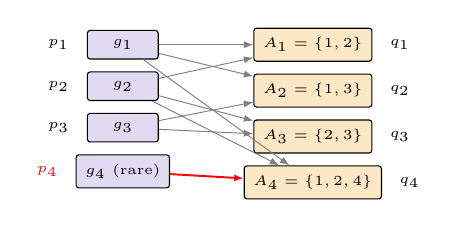
\begin{tikzpicture}[
   node distance=1.5mm,
   grp/.style={draw,rounded corners=1pt,minimum width=9mm,minimum height=3.4mm,font=\tiny,fill=Periwinkle!20},
   atm/.style={draw,rounded corners=1pt,minimum width=13mm,minimum height=3.4mm,font=\tiny,fill=YellowOrange!20},
   e/.style={-{Latex[length=1.2mm]},gray,line width=.35pt},
   lbl/.style={font=\tiny\itshape}
]
\node[grp] (g1) {$g_1$};
\node[grp,below=of g1] (g2) {$g_2$};
\node[grp,below=of g2] (g3) {$g_3$};
\node[grp,below=of g3] (g4) {$g_4$ \tiny(rare)};

\node[atm,right=12mm of g1] (a1) {$A_1=\{1,2\}$};
\node[atm,below=of a1] (a2) {$A_2=\{1,3\}$};
\node[atm,below=of a2] (a3) {$A_3=\{2,3\}$};
\node[atm,below=of a3] (a4) {$A_4=\{1,2,4\}$};

\draw[e] (g1)--(a1); \draw[e] (g2)--(a1);
\draw[e] (g1)--(a2); \draw[e] (g3)--(a2);
\draw[e] (g2)--(a3); \draw[e] (g3)--(a3);
\draw[e] (g1)--(a4); \draw[e] (g2)--(a4); \draw[e,Red,line width=.7pt] (g4)--(a4);

\node[lbl,left=1mm of g1] {$p_1$};
\node[lbl,left=1mm of g2] {$p_2$};
\node[lbl,left=1mm of g3] {$p_3$};
\node[lbl,left=1mm of g4,Red] {$p_4$};
\node[lbl,right=1mm of a1] {$q_1$};
\node[lbl,right=1mm of a2] {$q_2$};
\node[lbl,right=1mm of a3] {$q_3$};
\node[lbl,right=1mm of a4] {$q_4$};
\end{tikzpicture}
\caption{The mask $E$: compositions carry the mass $q$ they occur with, groups
must receive the mass $p$ the objective assigns. Group $4$ is reachable only
through $A_4$, so alignment needs $p_4\le q_4$, the Hall condition of
Thm.~\ref{thm:feas} on $I=\{4\}$; a smaller batch deletes $A_4$ and makes
$p_4$ unreachable.}
\label{fig:mask}
\end{figure}

\noindent\textbf{When alignment is possible.}
Existence is a supply--demand question on the bipartite graph $E$, settled
by flow duality (proofs in the appendix).

\begin{theorem}[Feasibility, {\cite[Thm.~1]{rahimi2025fedavot}}]
\label{thm:feas}
For $I\subseteq\Nn{N}$ let $\mathcal{N}(I)=\{j:\exists\,i\in I,\ (i,j)\in E\}$
and $\mathcal{S}(I)=\{j: A_j\subseteq I\}$. Problem \eqref{eq:mot} is feasible
if and only if
\begin{equation}
\sum_{j\in\mathcal{S}(I)}q_j\;\le\;\sum_{i\in I}p_i\;\le\;\sum_{j\in\mathcal{N}(I)}q_j
\qquad\forall\,I\subseteq\Nn{N}.
\label{eq:hall}
\end{equation}
\end{theorem}

\begin{corollary}[Coverage law and severity]
\label{cor:batchsize}
Feasibility of \eqref{eq:mot} requires $\PP[A^t=\{i\}]\le p_i\le r_i$ for every
$i$, with $r_i$ the observation rate. Writing
\begin{equation}
\nu\;\triangleq\!\!\sum_{i\,:\,p_i>r_i}\!\! p_i
\label{eq:batchlaw}
\end{equation}
for the \emph{infeasible mass}, $\nu=0$ iff the upper constraints hold.
Under i.i.d.\ sampling of $b$ examples the upper constraint reads
$b\ge\log(1-p_i)/\log(1-\pi_i)$, under $K$-of-$N$ group sampling
$p_i\le K/N$; $\nu$ is the axis Sec.~\ref{sec:exp} sweeps.
\end{corollary}

\noindent\textbf{Computing the plan.}
Given feasibility, a coupling is obtained by Sinkhorn scaling on the masked
support \cite{sinkhorn1967,cuturi2013,peyre2019} (appendix, \eqref{eq:ipfp}),
$O(|E|)$ per sweep with $M$ the number of \emph{realized} compositions,
once, offline; training then adds one lookup and one multiply per group per
step. Since $\mathbf{1}_N^\top T=q$ and $Y=T\mathrm{diag}(q)^{-1}$, every
column $Y[\cdot,j]$ is a probability vector on $A_j$, the property each
bound uses. Algorithm~\ref{alg:gavot} is the resulting method; $\gamma=1$ is
the risk-neutral rule analyzed here, $\gamma<1$ the layer of Sec.~\ref{sec:cvar}.

\begin{algorithm}[t]
\caption{\avot{}: group-fair SGD by masked transport}
\label{alg:gavot}
\begin{algorithmic}[1]
\Require $p$; $(q,\{A_j\},E)$; $\eta$; $T$; $(\alpha,\gamma)$, $\gamma=1$ risk-neutral
\State $(T,Y)\leftarrow$ Sinkhorn scaling for $(p,q,E)$ \Comment{offline, once}
\State $\theta^0\in\mathcal{C}$, $\ t^0\in\R$
\For{$t=1,\dots,T$}
  \State draw batch $B^t$; set $A^t$, let $j(t)$ be s.t.\ $A_{j(t)}=A^t$
  \State $g^t_i \leftarrow$ stochastic subgradient of $f_i$ from $B^t\cap$ group $i$
  \State $w^t_i \leftarrow Y[i,j(t)]\big(\gamma+\tfrac{1-\gamma}{\alpha}\mathbf{1}\{\hat f^t_i>t^{t-1}\}\big)$
  \State $\theta^{t}\leftarrow\Proj\big(\theta^{t-1}-\eta\sum_{i\in A^t}w^t_i\,g^t_i\big)$
  \State $t^{t}\leftarrow t^{t-1}-\eta(1-\gamma)\big(1-\tfrac{1}{\alpha}\sum_{i\in A^t}Y[i,j(t)]\mathbf{1}\{\hat f^t_i>t^{t-1}\}\big)$
\EndFor
\Ensure $\bar\theta_T=\frac{1}{T}\sum_{t=1}^{T}\theta^t$
\end{algorithmic}
\end{algorithm}

\noindent\textbf{Analysis.}
Let $\hat g(\theta)=\sum_{i\in A^t}Y[i,j(t)]\,g_i(\theta)$ be the
transport-weighted batch subgradient of Algorithm~\ref{alg:gavot}. Everything
rests on \cite[Lem.~1]{rahimi2025fedavot} moved from models to gradients:
transport removes bias, it is not a variance reduction device.

\begin{lemma}[Unbiasedness]
\label{lem:unbiased}
Let $T$ satisfy \eqref{eq:mot}. Then $\E[\hat g(\theta)\mid\theta]\in\partial F_p(\theta)$
for every $\theta\in\mathcal{C}$.
\end{lemma}

\begin{lemma}[Second moment, free of coverage]
\label{lem:variance}
$\E\|\hat g(\theta)\|^2\le G^2$ for every $\theta\in\mathcal{C}$, with no
dependence on $|A^t|$ or on $N$.
\end{lemma}

\begin{theorem}[Rate]
\label{thm:rate}
Under Assumption~\ref{ass:std}, if \eqref{eq:mot} is feasible then
Algorithm~\ref{alg:gavot} with $\gamma=1$ and $\eta=D/(G\sqrt{T})$ satisfies
\begin{equation}
\E\big[F_p(\bar\theta_T)\big]-F_p(\theta^\star)\;\le\;\frac{DG}{\sqrt{T}} .
\label{eq:rate}
\end{equation}
The constant is that of full-participation SGD, independent of batch coverage.
\end{theorem}

\noindent\textbf{Outside the feasible region.}
When \eqref{eq:hall} fails, Sinkhorn accumulates at the coupling whose row
marginal $\hat p\triangleq T\mathbf{1}$ is KL-closest to $p$ over the
reachable polytope $\{T\mathbf{1}: T\ge 0,\ \mathbf{1}^\top T=q,\
\mathrm{supp}(T)\subseteq E\}$ \cite{csiszar1975,gietl2013ipfp,peyre2019}.
The column marginal is met exactly, so both lemmas hold with $\hat p$ for
$p$: unbiased SGD on the surrogate $F_{\hat p}$, with $\hat p_i\le r_i$ on
singletons, so groups with $p_i>r_i$ are truncated at their observation rate.

\begin{theorem}[Infeasible regime]
\label{thm:infeasible}
Let $\hat p$ be the row marginal of the Sinkhorn limit,
$\theta^\dagger\in\argmin_{\mathcal{C}}F_{\hat p}$, and write
$\Phi(w)\triangleq F_p\big(\argmin_{\mathcal{C}} F_w\big)$ for the $p$-risk of
the minimizer of the $w$-weighted risk. Then
\begin{equation}
\E\big[F_p(\bar\theta_T)\big]-F_p(\theta^\star)
\;=\;\underbrace{\Phi(\hat p)-\Phi(p)}_{\text{alignment floor}}
\;+\;\underbrace{\varepsilon_T(\hat p)}_{\text{optimization residual}} ,
\label{eq:infeasible}
\end{equation}
where $\varepsilon_T(\hat p)\triangleq\E F_p(\bar\theta_T)-F_p(\theta^\dagger)$
satisfies $\E F_{\hat p}(\bar\theta_T)-F_{\hat p}(\theta^\dagger)\le DG/\sqrt{T}$
and $\varepsilon_T(\hat p)\to 0$ whenever $\bar\theta_T\to\theta^\dagger$.
Group-blind averaging obeys \eqref{eq:infeasible} with $\tilde p$ in place of
$\hat p$. Writing $\Delta_{\mathrm{floor}}\triangleq\Phi(\tilde p)-\Phi(\hat p)$
for the \emph{alignment gain}, transport improves on group-blind averaging
exactly when $\Delta_{\mathrm{floor}}>\varepsilon_T(\hat p)-\varepsilon_T(\tilde p)$,
and every floor is bounded by $\Phi(w)-\Phi(p)\le 2M\|p-w\|_1$.
\end{theorem}
\noindent Both terms are available before training, $\hat p,\tilde p$ from
$(p,q,E)$ and $\Phi$ exactly on instances with a closed-form or convex
frontier; the gain decides the sign, the residual is a stepsize artifact
(Sec.~\ref{sec:exp}).


% =====================================================================
\section{A Risk-Averse Layer over Groups}
\label{sec:cvar}
% =====================================================================

Exact alignment delivers the $p$-weighted risk, an average, which can hide a
group. Where the requirement is on the worst group instead, we compose a
mean--CVaR functional over groups on top of the transport weights
\cite{rahimi2025agnostic,rockafellar2000cvar}:
\begin{equation}
F_p^{\alpha,\gamma}(\theta)\;\triangleq\;\gamma F_p(\theta)+(1-\gamma)\,
\CVaR^p_\alpha\big(f(\theta)\big),\quad \alpha,\gamma\in(0,1],
\label{eq:meancvar}
\end{equation}
where $\CVaR^p_\alpha$ is the conditional value at risk of the group-loss vector
under $p$. The Rockafellar--Uryasev representation turns \eqref{eq:meancvar}
into a joint minimization over $(\theta,t)$,
\begin{equation}
\Phi(\theta,t)=\gamma\sum_i p_i f_i(\theta)+(1-\gamma)\Big(t+\tfrac{1}{\alpha}
\sum_i p_i\big[f_i(\theta)-t\big]_+\Big),
\label{eq:ru}
\end{equation}
jointly convex, with subgradients in both arguments $p$-weighted sums of
per-group quantities, so Lemma~\ref{lem:unbiased} applies unchanged: transport
fixes \emph{which} distribution the expectation is under, CVaR \emph{what} is
averaged (lines 6 and 8 of Algorithm~\ref{alg:gavot}).

\begin{theorem}[Rate under mean--CVaR]
\label{thm:cvar}
Under the hypotheses of Theorem~\ref{thm:rate}, Algorithm~\ref{alg:gavot} with
$\eta=\Theta(1/\sqrt{T})$ satisfies
$\E[F_p^{\alpha,\gamma}(\bar\theta_T)]-\min F_p^{\alpha,\gamma}
=O\!\big(\kappa(\alpha,\gamma)/\sqrt{T}\big)$ with
$\kappa(\alpha,\gamma)=\gamma+(1-\gamma)/\alpha$. In the infeasible regime the
bound of Theorem~\ref{thm:infeasible} acquires the same factor on its
statistical term, the bias term being unchanged.
\end{theorem}

Both $\gamma=1$ and $\alpha=1$ recover Theorem~\ref{thm:rate} exactly; sending
$\alpha\downarrow 0$ drives \eqref{eq:meancvar} to the worst group at the cost
$\kappa(\alpha,\gamma)\to\infty$: the parameter prices robustness in the
convergence constant, not in the limit.

\begin{remark}[Relation to constrained learning]
\label{rem:penalty}
$\max_i f_i$ is the exact-penalty limit of $\min f_0$ s.t.\ $f_i\le c_i$, a
fixed price on the largest violation matching penalized and constrained values
once it exceeds the least $\ell_1$ norm on the dual-optimal set
\cite{rahimi2026exactpenalty}. The $\alpha\downarrow 0$ edge of
\eqref{eq:meancvar} is thus the scalarization a constrained specification
selects, with $\kappa$ its price in the rate.
\end{remark}

% =====================================================================
%  Section 5: Experiments.
% =====================================================================
\section{Experiments}
\label{sec:exp}

\noindent\textbf{Instances and protocol.}
\emph{Adult} income classification \cite{uci_adult}: logistic regression
($\eta{=}0.1$) on $100$ race-homogeneous groups of $30$ samples, groups per
race $\propto$ prevalence ($85/10/3/1/1$), target uniform over the five
races ($p_i=0.2$ for a smallest-race group). \emph{IMDb-Wiki} age
regression \cite{rothe2018imdbwiki}: linear regression (mean-squared
error, MSE) on $128$-d face embeddings ($\eta{=}10^{-2}$) over $100$ identities, cubic target
$p_i\propto(101-i)^3$. Observation rates are swept: Adult $r\propto
p^{\beta}$, $\beta\in\{0,\tfrac14,\tfrac12,\tfrac34,1\}$, from prevalence
($\nu{=}0.60$) to aligned ($\nu{=}0$); IMDb-Wiki $r_i\propto i^{\beta}$,
$\beta\in\{0,\tfrac12,1,\tfrac32,2,3\}$, from uniform ($\nu{=}0.31$) to the
mirror image of $p$ ($\nu{=}0.88$), plus aligned $r_i\propto 101-i$
($\nu{=}0$): eleven instances. Each step observes $K{=}3$ groups drawn
$\propto r$, each taking $H{=}5$ local steps before the weighted average: \avot{}; \emph{group-blind averaging}, uniform over
the observed groups ($\tilde p_i=r_i/K$); the \emph{fixed multiplier}
$m/K$; \emph{full}, every group every step weighted by $p$. Stepsize
$\eta_t=\eta/(1+t/1000)$, fixed before the comparison and shared by every
rule (faster decays widen the IMDb-Wiki gap, never flip a winner), $4000$
steps, $5$ seeds, $F_p$ over the last $500$ steps. Floors are exact.

% ----------------------------------------------------------- Table 1
\begin{table}[t]
\centering
\caption{Headline cells, tail-500 over $5$ seeds, decaying stepsize. \emph{full}:
every group every step; \emph{upsamp.}: weights $\propto p_i/r_i$ within the
batch; LDS \cite{yang2021dir}: label-distribution smoothing, regression only.
The fixed multiplier $m/K$ reaches $0.670$ and $8504$ on the two infeasible
instances and diverges on the aligned ones.}
\label{tab:overall}
\small\setlength{\tabcolsep}{3pt}
\begin{tabular}{lccccc}
\toprule
Instance & \avot{} & unif.\ avg & upsamp. & LDS & full \\
\midrule
Adult, $\nu{=}0.60$ & $\best{0.2269}$ & $0.2479$ & $0.2288$ & -- & $0.2073$ \\
Adult, $\nu{=}0$   & $0.2075$ & $0.2077$ & $0.2075$ & -- & $0.2073$ \\
IMDb, $\nu{=}0.31$  & $\best{86.06}$ & $91.63$ & $86.74$ & $94.28$ & $82.95$ \\
IMDb, $\nu{=}0$    & $\best{84.28}$ & $86.37$ & $84.40$ & $89.43$ & $82.95$ \\
\bottomrule
\end{tabular}
\vspace{-8pt}
\end{table}

% ----------------------------------------------------------- Fig 2
\begin{figure*}[t]
\centering
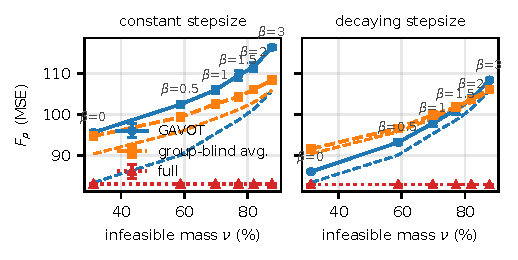
\includegraphics[width=\textwidth]{figs/severity_imdb.pdf}
\caption{IMDb-Wiki severity sweep: measured tail-500 (solid, $\pm1$ std)
against the exact floor $\Phi(\cdot)$ of each rule (dashed). Left, constant
stepsize: the residual swamps the alignment gain and transport loses
everywhere. Right, decaying: the curves track their floors and transport wins
until the floors close at high $\nu$.}
\vspace{-10pt}
\label{fig:severity}
\end{figure*}

\begin{figure*}[t]
\centering

\includegraphics[width=\textwidth]{figs/rare_group_fit.pdf}
\caption{Loss on the least represented group, decaying stepsize: Adult,
cross-entropy on race Other ($p_i=0.2$) against the observation exponent;
IMDb-Wiki, MSE on the $20$ top-importance identities, the least observed
once $\beta>0$. Same runs as Table~\ref{tab:overall}.}
\vspace{-10pt}
\label{fig:rare}
\end{figure*}

\noindent\textbf{E1: the headline cells.}
Table~\ref{tab:overall} reports the four headline instances. Transport wins
on three: Adult under prevalence availability,
$0.2269$ against $0.2479$ ($t{=}45$), and both IMDb cells, $86.06$ against
$91.63$ ($t{=}21$) and $84.28$ against $86.37$ ($t{=}13$); on Adult aligned
the two coincide at the oracle value, as Proposition~\ref{prop:surrogate}
predicts when $\tilde p=p$. Self-normalized upsampling
recovers most of the gain and transport the rest ($t{=}5.8$, $2.6$ against it); downsampling never beats
it, and LDS, which reweights by label rarity rather than group observation,
trails even group-blind averaging. On the least represented group the
margin over upsampling widens ($77.0$ against $80.0$, $73.6$ against $75.6$
on IMDb-Wiki).

\noindent\textbf{E2: the least represented group.}
Fig.~\ref{fig:rare} reads the same runs on the group the target exists for.
On Adult, transport lowers the loss on race Other at every skew: $0.073$
against $0.119$ on the prevalence instance (full $0.031$), $0.031$ against
$0.035$ aligned, matching full. On IMDb-Wiki the top-importance identities show the crossover of
Table~\ref{tab:severity} one step earlier: transport wins at $\nu\le0.70$
($77.0$ against $86.4$ at $\nu{=}0.31$, full $72.2$; $73.6$ against $79.9$
aligned) and loses at the three most infeasible skews. The single most
starved group (largest $p_i/r_i$) is Other itself on Adult and the top
identity on IMDb-Wiki, $253$ against $331$ at $\nu{=}0.31$ (full $219$).

% ----------------------------------------------------------- Table 2
\begin{table}[t]
\centering
\caption{IMDb-Wiki severity sweep, decaying stepsize: $\Delta_{\mathrm{floor}}$
the alignment gain of Theorem~\ref{thm:infeasible}, \emph{gain} the measured
advantage of transport, $t$ its Welch statistic. The residual averages $1.9$;
the sign flips where $\Delta_{\mathrm{floor}}$ crosses it.}
\label{tab:severity}
\setlength{\tabcolsep}{3.0pt}
\begin{tabular}{ccccc}
\toprule
$\beta$ & $\nu$ & $\Delta_{\mathrm{floor}}$ & gain & $t$ \\
\midrule
$0$   & $0.31$ & $6.99$ & $\best{+5.57}$ & $20.7$ \\
$0.5$ & $0.59$ & $5.71$ & $\best{+3.46}$ & $11.3$ \\
$1.0$ & $0.70$ & $3.67$ & $\best{+2.05}$ & $5.4$ \\
$1.5$ & $0.77$ & $2.56$ & $+0.58$ & $1.1$ \\
$2.0$ & $0.82$ & $1.62$ & $-0.03$ & $-0.1$ \\
$3.0$ & $0.88$ & $0.02$ & $-2.28$ & $-7.9$ \\
\bottomrule
\end{tabular}
\vspace{-8pt}
\end{table}

\noindent\textbf{E3: the crossover, and where the sign comes from.}
On Adult (Table~\ref{tab:severity}, Fig.~\ref{fig:severity}) the measured gain tracks $\Delta_{\mathrm{floor}}$ within $4\%$ at
three of five skews and exceeds it at the two most infeasible ($0.0210$
against $0.0110$, $0.0181$ against $0.0144$). On IMDb-Wiki the gain sits below
the floor by a residual close to constant in $\beta$, mean $1.9$, and the
sign flips exactly where $\Delta_{\mathrm{floor}}$ crosses that value,
between $\beta{=}1.5$ ($2.56$, gain $+0.58$) and $\beta{=}2.0$ ($1.62$,
$-0.03$): Theorem~\ref{thm:infeasible} at finite $T$. The $\ell_1$ criterion
cannot: $\|p-\hat p\|_1<\|p-\tilde p\|_1$ in all eleven instances, the three
where transport loses or ties included.

\noindent\textbf{E4: why the sign flips.}
At constant stepsize (Fig.~\ref{fig:severity}, left) transport loses on all
six IMDb skews, by up to $7.9$. A
starved group has $p_i>r_i$, so $\hat p$ truncates at the observation rate;
as $\nu$ grows $\hat p$ and $\tilde p$ starve the same groups and the floors
converge ($\Delta_{\mathrm{floor}}$ from $6.99$ to $0.02$, both $105.9$ at
$\nu{=}0.88$). Transport still concentrates weight on a starved
group whenever it appears, so its variance about the mean is larger
(Lemma~\ref{lem:variance} bounds only the second moment), and at constant
stepsize the iterates sit on a noise floor proportional to it. Under
$\eta_t=\eta/(1+t/1000)$ that floor decays, the curves fall onto their
dashed floors, and what remains is the residual, $2.3$ at $\nu{=}0.88$, the
one significant loss.

\noindent\textbf{E5: risk aversion, and where it does not help.}
On a $10\times10$ $(\alpha,\gamma)$ grid the overall objective is minimized
on the $\gamma=1$ edge of every instance: risk aversion costs the average. It earns its keep once, on the worst race of
Adult under prevalence availability: \avotcvar{} at $(0.2,0.7)$ reaches
$0.3624$ against $0.3679$ for \avot{} and $0.3994$ for group-blind averaging. On the least represented group the layer
never helps: the grid's best rare-group loss is at $\gamma{=}1$ on all four
headline instances. CVaR tilts among the groups present in the batch, and the rare
group is absent from most; on top of transport it multiplies weights already
$p_i/r_i$ large and amplifies variance, not alignment.

% =====================================================================


% =====================================================================
\vspace{-4pt}
\section{Conclusion}
% =====================================================================

Group-fair training fails at one fixable place: the aggregation step, blind
to the weighting the objective declares. Reading a minibatch as a
partial-participation event makes the fix the masked transport problem of
federated learning, with its feasibility characterization, an $O(1/\sqrt{T})$
guarantee free of batch coverage, and a coverage law whose infeasible mass
$\nu$ orders instances by severity. Transport is worth applying while the
alignment gain exceeds the optimization residual, both computable before
training, and the residual is a stepsize artifact a decaying schedule removes;
the nonconvex case remains open.

% =====================================================================
\clearpage
\renewcommand{\refname}{REFERENCES}

\begin{thebibliography}{99}\setlength{\itemsep}{-2pt}\small

\bibitem{buolamwini2018gender}
J.~Buolamwini and T.~Gebru, ``Gender shades: Intersectional accuracy disparities
in commercial gender classification,'' in \emph{Proc. Conf. Fairness,
Accountability and Transparency (FAT*)}, 2018, pp. 77--91.

\bibitem{hashimoto2018repeated}
T.~Hashimoto, M.~Srivastava, H.~Namkoong, and P.~Liang, ``Fairness without
demographics in repeated loss minimization,'' in \emph{Proc. Int. Conf. Machine
Learning (ICML)}, 2018, pp. 1929--1938.

\bibitem{sagawa2020dro}
S.~Sagawa, P.~W. Koh, T.~Hashimoto, and P.~Liang, ``Distributionally robust
neural networks for group shifts,'' in \emph{Proc. Int. Conf. Learning
Representations (ICLR)}, 2020.

\bibitem{mohri2019agnostic}
M.~Mohri, G.~Sivek, and A.~T. Suresh, ``Agnostic federated learning,'' in
\emph{Proc. Int. Conf. Machine Learning (ICML)}, 2019, pp. 4615--4625.

\bibitem{li2020fair}
T.~Li, M.~Sanjabi, A.~Beirami, and V.~Smith, ``Fair resource allocation in
federated learning,'' in \emph{Proc. Int. Conf. Learning Representations
(ICLR)}, 2020.

\bibitem{rahimi2025fedavot}
H.~Rahimi and D.~Kalogerias, ``FedAVOT: Exact distribution alignment in
federated learning via masked optimal transport,'' in \emph{Proc. IEEE Int.
Conf. Acoustics, Speech and Signal Processing (ICASSP)}, 2026.

\bibitem{rahimi2025agnostic}
H.~Rahimi and D.~Kalogerias, ``Convergence of agnostic federated averaging,''
in \emph{Proc. IEEE Int. Workshop Computational Advances in Multi-Sensor
Adaptive Processing (CAMSAP)}, 2025.

\bibitem{wang2020objective}
J.~Wang, Q.~Liu, H.~Liang, G.~Joshi, and H.~V. Poor, ``Tackling the objective
inconsistency problem in heterogeneous federated optimization,'' in \emph{Adv.
Neural Inf. Process. Syst. (NeurIPS)}, vol.~33, 2020, pp. 7611--7623.

\bibitem{cho2022biased}
Y.~J. Cho, J.~Wang, and G.~Joshi, ``Towards understanding biased client
selection in federated learning,'' in \emph{Proc. Int. Conf. Artificial
Intelligence and Statistics (AISTATS)}, 2022, pp. 10351--10375.

\bibitem{mcmahan2017fedavg}
H.~B. McMahan, E.~Moore, D.~Ramage, S.~Hampson, and B.~A. y~Arcas,
``Communication-efficient learning of deep networks from decentralized data,''
in \emph{Proc. Int. Conf. Artificial Intelligence and Statistics (AISTATS)},
2017, pp. 1273--1282.

\bibitem{agarwal2018reductions}
A.~Agarwal, A.~Beygelzimer, M.~Dud\'{i}k, J.~Langford, and H.~Wallach, ``A
reductions approach to fair classification,'' in \emph{Proc. Int. Conf. Machine
Learning (ICML)}, 2018, pp. 60--69.

\bibitem{cotter2019twoplayer}
A.~Cotter, H.~Jiang, and K.~Sridharan, ``Two-player games for efficient
non-convex constrained optimization,'' in \emph{Proc. Int. Conf. Algorithmic
Learning Theory (ALT)}, 2019, pp. 300--332.

\bibitem{chamon2020pacc}
L.~F.~O. Chamon and A.~Ribeiro, ``Probably approximately correct constrained
learning,'' in \emph{Adv. Neural Inf. Process. Syst. (NeurIPS)}, vol.~33, 2020,
pp. 16722--16735.

\bibitem{chamon2023nonconvex}
L.~F.~O. Chamon, S.~Paternain, M.~Calvo-Fullana, and A.~Ribeiro, ``Constrained
learning with non-convex losses,'' \emph{IEEE Trans. Inf. Theory}, vol.~69,
no.~3, pp. 1739--1760, 2023.

\bibitem{rahimi2026exactpenalty}
H.~Rahimi, S.~Pougkakiotis, and D.~Kalogerias, ``An exact penalty method for
constrained statistical learning over universal RKHSs,'' 2026, submitted.
%%FILLIN: replace with the arXiv number once posted.

\bibitem{rizk2021importance}
M.~Rizk, S.~Vlaski, and A.~H. Sayed, ``Optimal importance sampling for
federated learning,'' in \emph{Proc. IEEE Int. Conf. Acoustics, Speech and
Signal Processing (ICASSP)}, 2021, pp. 3110--3114.

\bibitem{katharopoulos2018not}
A.~Katharopoulos and F.~Fleuret, ``Not all samples are created equal: Deep
learning with importance sampling,'' in \emph{Proc. Int. Conf. Machine
Learning (ICML)}, 2018, pp. 2525--2534.

\bibitem{sinkhorn1967}
R.~Sinkhorn, ``Diagonal equivalence to matrices with prescribed row and column
sums,'' \emph{Amer. Math. Monthly}, vol.~74, no.~4, pp. 402--405, 1967.

\bibitem{cuturi2013}
M.~Cuturi, ``Sinkhorn distances: Lightspeed computation of optimal transport,''
in \emph{Adv. Neural Inf. Process. Syst. (NeurIPS)}, vol.~26, 2013, pp.
2292--2300.

\bibitem{peyre2019}
G.~Peyr\'{e} and M.~Cuturi, \emph{Computational Optimal Transport}. Now
Publishers, 2019.

\bibitem{gietl2013ipfp}
C.~Gietl and F.~P. Reffel, ``Accumulation points of the iterative proportional
fitting procedure,'' \emph{Statistics}, vol.~47, no.~6, pp. 1321--1335, 2013.

\bibitem{csiszar1975}
I.~Csisz\'{a}r, ``$I$-divergence geometry of probability distributions and
minimization problems,'' \emph{Ann. Probab.}, vol.~3, no.~1, pp. 146--158, 1975.

\bibitem{hall1935}
P.~Hall, ``On representatives of subsets,'' \emph{J. London Math. Soc.},
vol.~10, no.~1, pp. 26--30, 1935.

\bibitem{fordfulkerson1956}
L.~R. Ford and D.~R. Fulkerson, ``Maximal flow through a network,'' \emph{Canad.
J. Math.}, vol.~8, pp. 399--404, 1956.

\bibitem{villani2009}
C.~Villani, \emph{Optimal Transport: Old and New}. Springer, 2009.

\bibitem{rockafellar2000cvar}
R.~T. Rockafellar and S.~Uryasev, ``Optimization of conditional value-at-risk,''
\emph{J. Risk}, vol.~2, no.~3, pp. 21--41, 2000.

\bibitem{curi2020adaptive}
S.~Curi, K.~Y. Levy, S.~Jegelka, and A.~Krause, ``Adaptive sampling for
stochastic risk-averse learning,'' in \emph{Adv. Neural Inf. Process. Syst.
(NeurIPS)}, vol.~33, 2020, pp. 1036--1047.

\bibitem{levy2020large}
D.~Levy, Y.~Carmon, J.~C. Duchi, and A.~Sidford, ``Large-scale methods for
distributionally robust optimization,'' in \emph{Adv. Neural Inf. Process.
Syst. (NeurIPS)}, vol.~33, 2020, pp. 8847--8860.

\bibitem{namkoong2017variance}
H.~Namkoong and J.~C. Duchi, ``Variance-based regularization with convex
objectives,'' in \emph{Adv. Neural Inf. Process. Syst. (NeurIPS)}, vol.~30,
2017, pp. 2971--2980.

\bibitem{nemirovski2009}
A.~Nemirovski, A.~Juditsky, G.~Lan, and A.~Shapiro, ``Robust stochastic
approximation approach to stochastic programming,'' \emph{SIAM J. Optim.},
vol.~19, no.~4, pp. 1574--1609, 2009.

\bibitem{li2020fedprox}
T.~Li, A.~K. Sahu, M.~Zaheer, M.~Sanjabi, A.~Talwalkar, and V.~Smith,
``Federated optimization in heterogeneous networks,'' in \emph{Proc. Machine
Learning and Systems (MLSys)}, 2020, pp. 429--450.

\bibitem{karimireddy2020scaffold}
S.~P. Karimireddy, S.~Kale, M.~Mohri, S.~J. Reddi, S.~U. Stich, and A.~T.
Suresh, ``SCAFFOLD: Stochastic controlled averaging for federated learning,''
in \emph{Proc. Int. Conf. Machine Learning (ICML)}, 2020, pp. 5132--5143.

\bibitem{uci_adult}
B.~Becker and R.~Kohavi, ``Adult,'' UCI Machine Learning Repository, 1996.

\bibitem{yang2021dir}
Y.~Yang, K.~Zha, Y.-C. Chen, H.~Wang, and D.~Katabi, ``Delving into deep
imbalanced regression,'' in \emph{Proc. Int. Conf. Machine Learning (ICML)},
2021.

\bibitem{rothe2018imdbwiki}
R.~Rothe, R.~Timofte, and L.~Van~Gool, ``Deep expectation of real and apparent
age from a single image without facial landmarks,'' \emph{Int. J. Comput.
Vis.}, vol.~126, no.~2--4, pp. 144--157, 2018.

\bibitem{theodoropoulos2024restricted}
P.~Theodoropoulos, K.~E. Nikolakakis, and D.~Kalogerias, ``Federated learning
under restricted user availability,'' in \emph{Proc. IEEE Int. Conf. Acoustics,
Speech and Signal Processing (ICASSP)}, 2024.

\end{thebibliography}

\clearpage
% =====================================================================
%  Appendix (one page). Standalone block: nothing in main.tex references it.
%  Paste after the bibliography if the venue permits an appendix page.
% =====================================================================
\appendix
\section{Appendix}

\noindent\textbf{A. Proofs.}
\emph{Theorem~\ref{thm:feas} (sketch).} Route supply $p_i$ from a source through group $i$, along the edges of $E$
with infinite capacity, into composition $j$ with demand $q_j$, and to a sink.
A coupling exists iff the maximum flow saturates every source edge, which by
max-flow/min-cut \cite{fordfulkerson1956} is the right inequality of
\eqref{eq:hall}; the left one is the same statement for the reversed network.
On singletons \eqref{eq:hall} is Hall's condition \cite{hall1935}.

\noindent\emph{Corollary~\ref{cor:batchsize}.} For $I=\{i\}$, $\mathcal{N}(I)$ is the set of compositions containing $i$, of
total mass $r_i$, and $\mathcal{S}(I)=\{j:A_j=\{i\}\}$. Substitute
$r_i=1-(1-\pi_i)^b$ and $r_i=K/N$.

\noindent\emph{Theorem~\ref{thm:rate}.} By non-expansiveness of $\Proj$,
$\|\theta^{t}-\theta^\star\|^2\le\|\theta^{t-1}-\theta^\star\|^2
-2\eta\langle\hat g^t,\theta^{t-1}-\theta^\star\rangle+\eta^2\|\hat g^t\|^2$.
Conditioning on $\theta^{t-1}$, Lemma~\ref{lem:unbiased} and convexity bound
the inner product below by $F_p(\theta^{t-1})-F_p(\theta^\star)$, and
Lemma~\ref{lem:variance} bounds the last term by $\eta^2G^2$. Summing,
telescoping, and applying Jensen to $\bar\theta_T$ gives
$\E F_p(\bar\theta_T)-F_p(\theta^\star)\le D^2/(2\eta T)+\eta G^2/2$, and the
stated $\eta$ balances the two terms \cite{nemirovski2009}.
In full: $\E\|\theta^{t}-\theta^\star\|^2\le\E\|\theta^{t-1}-\theta^\star\|^2-2\eta\,\E[F_p(\theta^{t-1})-F_p(\theta^\star)]+\eta^2G^2$;
summing over $t\le T$, telescoping, dropping the terminal distance and applying Jensen to $\bar\theta_T$ gives
$\E F_p(\bar\theta_T)-F_p(\theta^\star)\le D^2/(2\eta T)+\eta G^2/2$, which is $DG/\sqrt{T}$ at $\eta=D/(G\sqrt{T})$;
the same bound holds for $\eta_t=\eta_0/\sqrt{t}$ up to constants.

\noindent\emph{Theorem~\ref{thm:infeasible}.} Add and subtract $F_p(\theta^\dagger)=\Phi(\hat p)$; the floor is exact by
definition and $\Phi(p)=F_p(\theta^\star)$. Theorem~\ref{thm:rate} applied to
$F_{\hat p}$ gives the residual bound on the surrogate; the residual on $F_p$
differs from it by $(F_p-F_{\hat p})(\bar\theta_T)-(F_p-F_{\hat p})(\theta^\dagger)$,
which vanishes as $\bar\theta_T\to\theta^\dagger$ (for instance under strong
convexity, which both of our instances satisfy). The $\ell_1$ bound is the
two-point argument of Proposition~\ref{prop:surrogate} with $w$ for $\tilde p$.

\medskip
\noindent\textbf{B. The infeasible regime in closed form (IMDb-Wiki, $\beta=3$).}
On the mirrored instance, where $41$ of $100$ groups violate $p_i\le r_i$ and hold
$88\%$ of the importance mass, the Sinkhorn limit truncates the target at the
observation-rate ceiling, $\hat p_i\approx\min(p_i,r_i)$ up to renormalization
(maximum deviation $0.023$), giving $\|p-\hat p\|_1=1.58$ of a maximum possible $2$.
Because the task is linear regression, the minimizers $\theta^\star$ of $F_p$ and
$\theta^\dagger$ of $F_{\hat p}$ are available in closed form:
$\Phi(p)=F_p(\theta^\star)=82.9$ (matching the measured full-coverage plateau, $82.95$)
and $\Phi(\hat p)=F_p(\theta^\dagger)=105.9$. The alignment floor is therefore
$23.0$, and the realized bias equals its exact expression
$|(p-\hat p)^\top L(\theta^\dagger)|=30.7$, where $L(\theta)$ collects the per-group
risks. The $\ell_1$ form $2M\|p-\hat p\|_1$ of Theorem~\ref{thm:infeasible} holds but is
conservative here, since any uniform bound satisfies $M\ge\max_i L_i(\theta^\dagger)\approx 454$.
The group-blind surrogate $\tilde p_i=r_i/K$ has the same floor to two decimals
($\Phi(\tilde p)=105.9$): both surrogates starve the same groups, which is why
$\Delta_{\mathrm{floor}}$ vanishes at this endpoint of Table~\ref{tab:severity}.

\medskip
\noindent\textbf{C. Adult severity sweep.} The five Adult skews omitted from
Table~\ref{tab:severity}, same conventions.
\begin{center}\footnotesize\setlength{\tabcolsep}{4pt}
\begin{tabular}{ccccc}
\toprule
$\beta$ & $\nu$ & $\Delta_{\mathrm{floor}}$ & gain & $t$ \\
\midrule
$0$    & $.60$ & $.0110$ & $\best{+.0210}$ & $44.7$ \\
$0.25$ & $.60$ & $.0144$ & $\best{+.0181}$ & $69.4$ \\
$0.5$  & $.40$ & $.0129$ & $\best{+.0134}$ & $35.2$ \\
$0.75$ & $0$   & $.0049$ & $\best{+.0050}$ & $35.8$ \\
$1$    & $0$   & $.0003$ & $+.0002$ & $7.1$ \\
\bottomrule
\end{tabular}
\end{center}

\medskip
\noindent\textbf{D. Adult per-race cross-entropy, prevalence regime.}
Tail-500 over $5$ seeds, decaying stepsize.
\begin{center}\footnotesize\setlength{\tabcolsep}{4pt}
\begin{tabular}{lccccc}
\toprule
 & White & Black & Asian-Pac. & Amer-Ind. & Other \\
\midrule
\avot{}            & $.339$ & $\best{.179}$ & $\best{.368}$ & $\best{.175}$ & $\best{.073}$ \\
group-blind avg.   & $\best{.332}$ & $.200$ & $.399$ & $.189$ & $.119$ \\
full               & $.379$ & $.177$ & $.328$ & $.123$ & $.031$ \\
\bottomrule
\end{tabular}
\end{center}
Transport improves four of five categories and regresses only the majority group,
the expected effect of reweighting toward a category-uniform target; the residual
loss on the two smallest categories is the unreachable mass of Cor.~\ref{cor:batchsize}.

\end{document}
